\documentclass{ximera}
  \outcome{Determine whether a linear approximation is an over- or under-approximation}
  \outcome{Understand the derivative as a linear approximation}
\begin{document}
\begin{problem}

  Shown below is the graph of $y = e^x$ and a tangent line $y = mx + b$ to the graph passing through the point $(8,e^8)$.
  \begin{image}
    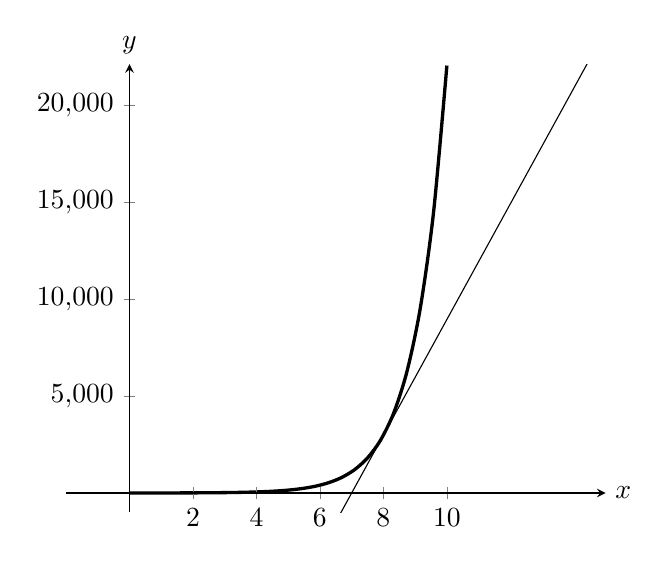
\begin{tikzpicture}
      \begin{axis}[
        clip=true,
        domain=0:10,
        ytickmin=0,ytickmax=20000,
        xtickmin=0,xtickmax=10,
        ymin=-1000, ymax=22100,
        xmin=-2, xmax=15,
        ytick={5000,10000,15000,20000},
        scaled y ticks=false,
        xlabel=$x$, ylabel=$y$,
        axis lines=center,
        every axis y label/.style={at=(current axis.above origin),anchor=south},
        every axis x label/.style={at=(current axis.right of origin),anchor=west},
        axis on top,
        ]          
        \addplot [very thick,smooth] {exp(x)};
        \addplot [smooth,domain=0:15] {exp(8)*(x-8) + exp(8)};
      \end{axis}
    \end{tikzpicture}  
  \end{image}
  How does $200m + b$ compare to $e^{200}$?
  \begin{multipleChoice}
    \choice{$200m + b$ equals $e^{200}$.}
    \choice{$200m + b$ is bigger than $e^{200}$.}
    \choice{$200m + b$ is a little bit smaller than $e^{200}$.}
    \choice[correct]{$200m + b$ is much smaller than $e^{200}$.}
  \end{multipleChoice}
\end{problem}
\end{document}
